% \IUref{IUAdmPS}{Administrar Planta de Selección}
% \IUref{IUModPS}{Modificar Planta de Selección}
% \IUref{IUEliPS}{Eliminar Planta de Selección}

% 


% Copie este bloque por cada caso de uso:
%-------------------------------------- COMIENZA descripción del caso de uso.
%\begin{figure}[htbp!]
	%	\centering
		%	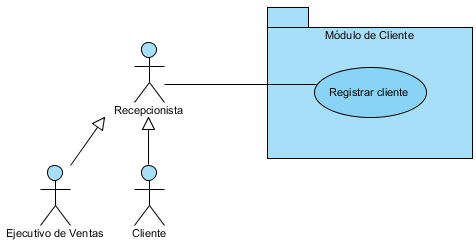
\includegraphics[width=0.8\textwidth]{images/RegistrarCliente}
		%\caption{Diagrama de Casos de Uso del sistema.}
	%\end{figure}

%\begin{UseCase}[archivo de imágen]{UCX}{Nombre del Caso de uso}{
	\begin{UseCase}{CU1}{Registrar cliente.}{
		Permite registrar los datos de un cliente mayor de 18 años para poder adquirir
una membresía. El registro de la información del cliente sólo lo podrá realizar la recepcionista, ejecutivo de ventas y el propio cliente.
	}
		\UCitem{Versión}{1.1}
		\UCitem{Actor}{Ejecutivo de Ventas, Recepcionista y Cliente.}
		\UCitem{Propósito}{Tener un historial sobre las membresías y/o servicios contratados por el cliente en el momento que se desee.}
		\UCitem{Entradas}{Nombre(s), Apellido Paterno, Apellido Materno, Fecha de Nacimiento, CURP, RFC, Sexo, Calle, Número exterior, Número interior, Colonia, Estado, Delegación/Municipio, Código Postal, Calle anterior, calle Posterior, Referencias, Correo electrónico, Teléfonos, Tipo de sangre, Enfermedades, Condición médica.}
		\UCitem{Origen}{Teclado}
		\UCitem{Salidas}{Mensaje de registro exitoso, número de cliente, envío de correo electrónico de confirmación a la cuenta de correo del cliente, muestra la \IUref{IU8}{Pantalla de cotización.}}
		\UCitem{Destino}{Servidor de correo, pantalla.}
		\UCitem{Precondiciones}{No tener registrado otro cliente con la misma CURP y contar con la mayoría de edad (+18).}
		\UCitem{Postcondiciones}{Habrá un cliente más registrado en el sistema.}
		\UCitem{Errores}{{\bf E1:} ``El cliente es menor de edad.'' -- El sistema muestra el Mensaje {\bf MSG1-}``Debes ser mayor de 18 años para continuar con el registro y adquirir tú membresía. Una vez finalizado el registro podrás dar de alta a un afiliado menor de edad'' y continua al paso 3.
		
		{\bf E2:} ``Existe un registro con la misma CURP.'' -- El sistema muestra el Mensaje {\bf MSG2-}``Este registro ya existe. Ingresa una nueva CURP o consulta los clientes y/o empleados registrados.'' y continua al paso 3.
		
		{\bf E3:} ``No se ingresaron todos los campos obligatorios.'' -- El sistema muestra el Mensaje {\bf MSG3-}``Ingresa los campos obligatorios marcados con * para continuar'' y continua al paso 3.
				
				{\bf E4:} ``El formato del dato es incorrecto''. -- El sistema muestra el Mensaje {\bf MSG4-}``Ingresa el valor correcto de acuerdo al formato que aparece en el campo'' y continua en el paso 3.}
		\UCitem{Tipo}{Caso de uso que extiende del \UCref{CU31}}
		\UCitem{Observaciones}{}
		\UCitem{Autor}{Roberto Mendoza Saavedra.}
		\UCitem{Revisor}{Francisco García Enríquez}
	\end{UseCase}

	\begin{UCtrayectoria}{Principal}
		\UCpaso[\UCactor] Solicita el ingreso al apartado de clientes seleccionando la opción ``Clientes'' de la \IUref{IU6}{Pantalla de perfil de empleado} \Trayref{A}.
		\UCpaso Muestra las operaciones disponibles para el actor mediante la \IUref{IU7}{Pantalla de operaciones del empleado.}
		\UCpaso[\UCactor] Solicita el registro de un nuevo cliente seleccionando la opción ``Registrar'' de la \IUref{IU7}{Pantalla de operaciones del empleado.}
		\UCpaso Solicita los datos del cliente a registrar mostrando la \IUref{IU3}{Pantalla de Registrar Cliente.}
		\UCpaso[\UCactor] Proporciona los datos personales de acuerdo a la \IUref{IU3}{Pantalla de Registrar Cliente.}
		\UCpaso Verifica la mayoría de edad del cliente [E1].
		\UCpaso Carga los estados de la república.
		\UCpaso[\UCactor] Proporciona los demás datos de la ubicación de acuerdo a la \IUref{IU3}{Pantalla de Registrar Cliente.}
		\UCpaso[\UCactor] Proporciona los datos de contacto de acuerdo a la \IUref{IU3}{Pantalla de Registrar Cliente.}
		\UCpaso[\UCactor] Proporciona los datos médicos de acuerdo a la \IUref{IU3}{Pantalla de Registrar Cliente.}
		\UCpaso[\UCactor] Confirma el registro de datos presionando el botón \IUbutton{Guardar} de la \IUref{IU3}{Pantalla de Registrar Cliente.}
		\UCpaso Verifica que todos los campos marcados como obligatorios en la \IUref{IU3}{Pantalla de Registrar Cliente} se hayan ingresado [E3].
		\UCpaso Verifica que todos los datos proporcionados tengan el formato especificado en el modelo de entidades de acuerdo al tipo de dato de cada campo [E4].
		\UCpaso Valida que no exista previamente un registro de cliente con la misma CURP [E2].
		\UCpaso Registra todos los datos proporcionados del cliente y muestra el Mensaje {\bf MSG16-}``Registro exitoso. Tú número de cliente es: [{\em Número de cliente}]'' \Trayref{B}.
		\UCpaso Direcciona a la \IUref{IU8}{Pantalla de cotización.}
\end{UCtrayectoria}

\begin{UCtrayectoriaA}{A}{El actor que realizará el nuevo registro será el propio cliente.}
			\UCpaso[\UCactor] Solicita su registro de datos seleccionando la opción ``Regístrate ya'' de la \IUref{IU1}{Página principal.}
			\UCpaso Solicita los datos del cliente mediante la \IUref{IU3}{Pantalla de Registrar Cliente} y continúa en el paso 5.		
		\end{UCtrayectoriaA}
		
		\begin{UCtrayectoriaA}{B}{El propio cliente concluye su proceso de registro.}
			\UCpaso Registra todos los datos proporcionado por el cliente y muestra el Mensaje {\bf MSG17-}``Registro exitoso. Tú número de cliente es: [{\em Número de cliente}]. Ahora, puedes cotizar la membresía que mejor se adapte a lo que buscas...COTÍZALA y acude a tú sucursal más cercana.'' 
			\UCpaso Direcciona a la \IUref{IU8}{Pantalla de cotización.}
		\end{UCtrayectoriaA}


			
%-------------------------------------- TERMINA descripción del caso de uso.